% TP5, Grupo 11. Actualizado contra código y figuras disponibles: 13/11/2026.
% Compilar: pdflatex document.tex (dos veces).
% Fuente matemática ED: EventPrediction.cpp y SimulationEDMD.cpp.
% Fuente matemática híbrido: SimulationHybrid.cpp; no thoughtsH.md (era propuesta).
% Fuentes de resultados: PNG y *_resumen.csv de esta carpeta; no se recalcularon datos.
% Exposición de 13 min: intro 1:00; implementación 5:00; simulaciones 1:30;
% resultados 5:00; conclusiones 0:30. Separadores: solo transición.
% Las diapositivas de apoyo se ubican después de las conclusiones.
% Observación pendiente: consignar equipo/compilación reales de las mediciones.
% Los MP4 locales se activan sobre la imagen en un visor PDF compatible.
% No se comprobó su reproducción en el equipo del aula. No usar externalviewer.
% Para entregar: activar entrega y completar URLs públicas (YouTube/Vimeo).
\documentclass[aspectratio=169,20pt]{beamer}
\geometry{paperwidth=320mm,paperheight=180mm}
\usepackage[utf8]{inputenc}
\usepackage[T1]{fontenc}
\usepackage{lmodern}
\usefonttheme{professionalfonts}
\usefonttheme[onlymath]{serif}
\usepackage[spanish,es-nodecimaldot]{babel}
\usepackage{amsmath,amssymb,graphicx,booktabs,tikz,multimedia}
\usetikzlibrary{arrows.meta,positioning,calc}
\usetheme{Frankfurt}
\usecolortheme{beaver}
\definecolor{darkred}{RGB}{153,0,0}
\definecolor{TS}{RGB}{214,39,40}
\definecolor{ED}{RGB}{31,119,180}
\definecolor{HY}{RGB}{148,103,189}
\setbeamercolor{frametitle}{bg=gray!8,fg=darkred}
\setbeamercolor{title}{fg=darkred}
\setbeamercolor{structure}{fg=darkred}
\setbeamercolor{section in head/foot}{bg=darkred,fg=white}
\setbeamertemplate{navigation symbols}{}
\setbeamertemplate{blocks}[default]
\setbeamersize{text margin left=12mm,text margin right=12mm}
\setbeamerfont{frametitle}{size=\fontsize{28}{33}\selectfont}
\setbeamerfont{title}{size=\fontsize{34}{40}\selectfont}
\newif\ifapoyo\apoyofalse
\newif\ifentrega\entregafalse
\newif\ifincluirapoyo\incluirapoyotrue
\newcommand{\urlTS}{}
\newcommand{\urlED}{}
\newcommand{\urlHY}{}
\setbeamertemplate{headline}{\begin{beamercolorbox}[wd=\paperwidth,ht=7mm,dp=2mm,leftskip=12mm]{section in head/foot}\fontsize{15}{18}\selectfont\insertsectionhead\end{beamercolorbox}}
\setbeamertemplate{footline}{\hbox{\begin{beamercolorbox}[wd=.85\paperwidth,ht=6mm,dp=2mm,leftskip=12mm]{section in head/foot}\fontsize{13}{16}\selectfont Grupo 11\quad Dinámica peatonal\end{beamercolorbox}\begin{beamercolorbox}[wd=.15\paperwidth,ht=6mm,dp=2mm,rightskip=8mm plus1fil]{section in head/foot}\fontsize{13}{16}\selectfont\ifapoyo Apoyo\else\insertpagenumber/\pageref{finprincipal}\fi\end{beamercolorbox}}}
\setbeamertemplate{itemize items}[circle]
\setlength{\parskip}{4mm}
\newcommand{\vb}[1]{\mathbf{#1}}
\newcommand{\un}[1]{\,\mathrm{#1}}
\newcommand{\notaBreve}[1]{{\fontsize{18}{22}\selectfont #1}}
\newcommand{\cita}{\vfill\notaBreve{Baglietto y Parisi, Physical Review E 83 (2011)}}
\newcommand{\grafico}[3]{\begin{frame}{#1}\notaBreve{#3}\par\vspace{1mm}\centering\includegraphics[width=.98\textwidth,height=.78\textheight,keepaspectratio]{#2}\end{frame}}
\newcommand{\video}[4]{\begin{frame}{#1}\centering\ifentrega
  \includegraphics[width=.98\textwidth,height=.78\textheight,keepaspectratio]{#2}\par
  \ifx#4\empty\notaBreve{\textcolor{magenta}{(insertar link)}}\else\notaBreve{\expandafter\url\expandafter{#4}}\fi
  \else\movie[poster,showcontrols]{\includegraphics[width=.98\textwidth,height=.78\textheight,keepaspectratio]{#2}}{#3}\par\notaBreve{\textcolor{magenta}{(insertar link)}}\fi\end{frame}}
\tikzset{bloque/.style={draw=darkred,thick,align=center,minimum height=15mm,text width=65mm},flecha/.style={->,very thick,>=Stealth}}
\AtBeginSection[]{\begin{frame}\centering\usebeamerfont{title}\textcolor{darkred}{\insertsectionhead}\end{frame}}
\title{Dinámica peatonal}
\subtitle{Evacuación: TSDMD, EDMD e híbrido}
\author{Grupo 11\\Santiago Diaz -- 63058\quad Lautaro Gazzaneo -- 61484\\Luca Maximiliano Rossi -- 63730}
\institute{Simulación de Sistemas -- ITBA}
\date{13 de noviembre de 2026}
\begin{document}
\begin{frame}\titlepage\end{frame}

\section{Introducción}
\begin{frame}{CPM: movimiento libre y recuperación}
\[
 \widehat{\vb e}_i=\frac{\vb q_i-\vb x_i}{\|\vb q_i-\vb x_i\|},\qquad
 v_d(r)=v_d^{\max}\left(\frac{r-r_{\min}}{r_{\max}-r_{\min}}\right)^\beta
\]
\vspace{3mm}
\[
 r_i^{n+1}=\min\!\left(r_{\max},r_i^n+\frac{r_{\max}}{\tau}\Delta t\right),\qquad
 \vb v_i^{n+1}=v_d(r_i^{n+1})\widehat{\vb e}_i
\]
\[
 \vb x_i^{n+1}=\vb x_i^n+\vb v_i^{n+1}\Delta t,\qquad
 \Delta t=\frac{r_{\min}}{2\max(v_d^{\max},v_e)}
\]
\notaBreve{$\vb x_i$: posición; $\vb q_i$: target; $r_i$: radio; $\tau$: recuperación; $\beta$: exponente.}
\end{frame}

\begin{frame}{CPM: contacto, contracción y escape}
\[
 \mathcal C_i=\{j:\|\vb x_i-\vb x_j\|\le r_i+r_j\},\qquad
 \mathcal W_i=\{w:\|\vb x_i-\vb p_{iw}\|\le r_i\}
\]
\[
 \vb s_i=\sum_{j\in\mathcal C_i}\frac{\vb x_i-\vb x_j}{\|\vb x_i-\vb x_j\|}
 +\sum_{w\in\mathcal W_i}\frac{\vb x_i-\vb p_{iw}}{\|\vb x_i-\vb p_{iw}\|}
\]
\[
 r_i^{n+1}=r_{\min},\qquad \vb v_i^{n+1}=v_e\frac{\vb s_i}{\|\vb s_i\|}
\]
\notaBreve{$j\ne i$; $\vb p_{iw}$: punto más cercano del segmento de pared.}
\end{frame}

\section{Implementación}
\begin{frame}{Tres motores, geometría y reglas compartidas}
\centering
\begin{tikzpicture}[node distance=18mm and 20mm]
\node[bloque,text=TS] (ts) {TSDMD\\paso CPM};
\node[bloque,right=of ts,text=HY] (hy) {Híbrido\\bolsa TS + vuelos ED};
\node[bloque,right=of hy,text=ED] (ed) {EDMD\\agenda de eventos};
\node[bloque,below=25mm of ts] (rules) {Reglas CPM};
\node[bloque,below=25mm of hy] (geo) {Agentes, paredes\\y grillas};
\node[bloque,below=25mm of ed] (pred) {Trayectorias\\y predicción};
\draw[flecha] (ts)--(rules);\draw[flecha] (hy)--(geo);\draw[flecha] (ed)--(pred);
\draw[flecha] (hy.south west)--(rules.north east);
\draw[flecha] (hy.south east)--(pred.north west);
\end{tikzpicture}
\vspace{8mm}
\[
\text{TSDMD:}\quad\text{contactos}\;\longrightarrow\;(r^{n+1},\vb v^{n+1})\;\longrightarrow\;\vb x^{n+1}
\]
% No incluye postproceso ni I/O. Los tres motores comparten parámetros y Board;
% CpmRules.h se comparte entre TSDMD y TS del híbrido, no con la recuperación ED.
\end{frame}

\begin{frame}{EDMD: tres fases entre eventos}
\centering
\begin{tikzpicture}
\node[bloque,text width=50mm,text=ED] (f) at (0,0) {Libre\\$r=r_{\max}$\\$v=v_d^{\max}$};
\node[bloque,text width=50mm,text=TS] (e) at (9,0) {Escape\\$r=r_{\min}$\\$v=v_e$};
\node[bloque,text width=50mm,text=HY] (r) at (18,0) {Recuperación\\$r\rightarrow r_{\max}$\\$v\rightarrow v_d^{\max}$};
\draw[flecha] (f)--node[above]{contacto}(e);
\draw[flecha] (e)--node[above,align=center]{fin de $\Delta t$\\sin contacto}(r);
\draw[flecha] (r.south)--(18,-3)--node[below]{radio máximo}(0,-3)--(f.south);
\draw[flecha] (r.north) to[bend right=35] node[above]{nuevo contacto} (e.north);
\end{tikzpicture}
\vfill
\notaBreve{Contacto persistente al terminar el escape: nuevo escape de duración $\Delta t$.}
% Decisión propia: escape continuo de duración dt; un contacto nuevo puede
% reiniciarlo. No se aplican leyes de colisión elástica de discos duros.
\end{frame}

\begin{frame}{EDMD: recuperación continua integrada exactamente}
\[
 \alpha=\frac{r_{\max}}{\tau},\qquad T_r=\frac{r_{\max}-r_{\min}}{\alpha}=0{,}30\un{s},\qquad
 u=t-t_{\mathrm{rec}}
\]
\[
 r(u)=r_{\min}+\alpha u,\qquad
 v(u)=v_d^{\max}\left(\frac{u}{T_r}\right)^\beta\quad(0\le u\le T_r)
\]
\[
 S(u)=
 \frac{v_d^{\max}T_r}{\beta+1}\left(\frac{u}{T_r}\right)^{\beta+1}
\]
\[
 \vb x(t)=\vb x(t_0)+\widehat{\vb e}\,[S(t-t_{\mathrm{rec}})-S(t_0-t_{\mathrm{rec}})]
\]
\notaBreve{Dirección fija por tramo; un cambio de target no reinicia la recuperación.}
% Aclaración oral: es la adaptación continua implementada, distinta del CPM
% discreto. La trayectoria es rectilínea por tramo, con rapidez no constante.
\end{frame}

\begin{frame}{EDMD: predicción del próximo contacto}
\[
 g_{ij}(t)=\|\vb x_i(t)-\vb x_j(t)\|-r_i(t)-r_j(t)
\]
\begin{columns}[T]
\begin{column}{.49\textwidth}
\textcolor{ED}{Radios y velocidades constantes}
\[
 (\vb u\!\cdot\!\vb u)h^2+2(\vb p\!\cdot\!\vb u)h+\|\vb p\|^2-R^2=0
\]
\notaBreve{$\vb p=\vb x_i-\vb x_j$; $\vb u=\vb v_i-\vb v_j$; $R=r_i+r_j$.}
\par Primera raíz de entrada válida.
\end{column}
\begin{column}{.48\textwidth}
\textcolor{HY}{Durante recuperación}
\[
 B\ge v_i+v_j+\dot r_i+\dot r_j
\]
\[
 h=\max\!\left(\frac{g-\varepsilon_c/2}{B},\frac{2\varepsilon_p}{B}\right)
\]
\notaBreve{Avance acotado + bisección;\quad $\varepsilon_c=10^{-9}\un{m}$, $\varepsilon_p=10^{-6}\un{m}$.}
\end{column}
\end{columns}
\vfill\notaBreve{Paredes: distancia al segmento, incluidos extremos. Horizonte limitado al tramo válido.}
% El mínimo de avance introduce tolerancia espacial; no decir raíz exacta en
% recuperación ni ausencia absoluta de penetración. Tiempo de bisección 1e-12 s.
\end{frame}

\begin{frame}{EDMD: agenda y búsqueda local}
\centering
\begin{tikzpicture}[node distance=17mm]
\node[bloque] (a) {Próximo evento\\vigente};
\node[bloque,right=of a] (b) {Contactos simultáneos\\estado común};
\node[bloque,right=of b] (c) {Actualizar afectados\\y sus predicciones};
\draw[flecha] (a)--(b);\draw[flecha] (b)--(c);
\end{tikzpicture}
\[
 \nu_i^{\mathrm{evento}}=\nu_i^{\mathrm{actual}}\quad\text{para cada participante}
\]
\[
 R_{\mathrm{busq}}=2r_{\max}+\left(2v_{\max}+2\alpha\right)\Delta+\varepsilon_p
\]
\[
 \Delta=0{,}05\un{s},\qquad 2v_{\max}+2\alpha=4\un{m/s}
\]
\notaBreve{Grilla por ventanas de duración $\Delta$; predicciones de pares limitadas a esa ventana.}
% nu es versión del vuelo. Simultaneidad: eventos a menos de 1e-11 s del primero.
% La grilla se reconstruye periódicamente; no confundir Delta con dt de CPM.
\end{frame}

\begin{frame}{Híbrido: anticipación y bolsa TS}
\[
 \mathcal B_0=\{i:r_i<r_{\max}\ \text{o contacto actual}\}
\]
\[
 t_{ij}^{\mathrm{contacto}}\le t_n+k\Delta t
 \quad\Longrightarrow\quad i,j\in\mathcal B_0
\]
\centering
\begin{tikzpicture}[x=1cm,y=1cm]
\draw[flecha] (0,0)--(20,0) node[right]{$t$};
\foreach \x/\label in {1/t_n,8/{t_n+\Delta t},15/{t_n+2\Delta t}}{
\draw (\x,-.2)--(\x,.2);\node[below] at (\x,-.3){$\label$};}
\fill[ED] (5,0) circle (.13);\node[above,text=ED] at (5,.3){contacto previsto};
\node[above,text=TS] at (1,1.3){entrada a TS};
\draw[flecha,TS] (1,1.1)--(1,.3);
\end{tikzpicture}
\vfill\notaBreve{$k$: anticipación en pasos.\quad El cambio de esquema no aplica anticipadamente la contracción.}
% Incluye contactos con paredes. La clasificación real comprueba los vuelos
% tentativos de los TS recuperados y repite el cierre si aparecen nuevas semillas.
% k=0 existe en el barrido; evitar afirmar entrada estrictamente previa para k=0.
\end{frame}

\begin{frame}{Híbrido: cierre de la bolsa y contactos mixtos}
\[
 \mathcal B_{\ell+1}=\mathcal B_\ell\ \cup\
 \{i:\exists j\in\mathcal B_\ell,\ \|\vb x_i-\vb x_j\|\le d^*\}
\]
\[
 \mathcal B_{\ell+1}=\mathcal B_\ell\quad\Longrightarrow\quad\mathcal B_{\mathrm{TS}}
\]
\begin{columns}[c]
\begin{column}{.48\textwidth}\centering
\begin{tikzpicture}
\foreach \x/\c in {0/TS,2.7/TS,5.4/TS,10/ED}{\draw[fill=\c!20,draw=\c,very thick] (\x,0) circle (.65);}
\draw[flecha,TS] (.8,0)--(1.9,0);\draw[flecha,TS] (3.5,0)--(4.6,0);
\node[below] at (2.7,-1){cierre sucesivo};
\node[below,text=ED] at (10,-1){ED};
\end{tikzpicture}
\end{column}
\begin{column}{.49\textwidth}
\[
 d^*\ge2r_{\max}+2v_{\max}\Delta t=0{,}60\un{m}
\]
\notaBreve{Fuera del cierre, un par ED--TS no puede tocarse en el próximo paso.}
\end{column}
\end{columns}
% El dibujo ilustra pertenencia, no escala. v_max=1.5 m/s, radios <=0.25 m.
% La garantía supone cierre completo; cada miembro nuevo incorpora vecinos.
\end{frame}

\begin{frame}{Híbrido: salida de TS y sincronización}
\[
 \mathrm{TS}\to\mathrm{ED}:\quad r_i=r_{\max},\quad\mathcal C_i=\mathcal W_i=\varnothing,
 \quad i\notin\mathcal B_{\mathrm{TS}}
\]
\[
 \vb x_i(t_{n+1})=
 \begin{cases}
 \vb x_i(t_n)+\vb v_i^{n+1}\Delta t,&i\in\mathcal B_{\mathrm{TS}},\\[2mm]
 \vb x_i(t_0)+v_d^{\max}\widehat{\vb e}_i(t_{n+1}-t_0),&i\notin\mathcal B_{\mathrm{TS}}.
 \end{cases}
\]
\centering\vspace{5mm}
\textcolor{HY}{Un reloj común}\qquad $t_{n+1}=t_n+\Delta t$
\par\notaBreve{La implementación avanza cada tick, incluso si la bolsa está vacía.}
% Importante: no presentar el salto largo sugerido en thoughtsH como implementado.
% La condición i no pertenece a B incluye anticipación y cierre, también para
% vuelos tentativos. La etiqueta del estado escrito corresponde al paso realizado.
\end{frame}

\section{Simulaciones}
\begin{frame}{Sistema y parámetros}
\begin{columns}[c]
\begin{column}{.44\textwidth}\centering
\begin{tikzpicture}[x=13mm,y=13mm]
\draw[very thick] (0,0)--(0,6)--(6,6)--(6,0)--(3.4,0);
\draw[very thick] (0,0)--(2.6,0);
\draw[<->] (-.6,0)--node[left]{$L$}(-.6,6);
\draw[<->] (2.6,-.5)--node[below]{$d$}(3.4,-.5);
\draw[dashed] (0,-1.2)--(6,-1.2) node[right]{$y=-1\un{m}$};
\foreach \x/\y in {1/4,2/2,4/5,5/3,3/4,4.5/1.5}{\fill[ED] (\x,\y) circle (.10);}
\node at (3,6.5){Esquema sin escala};
\end{tikzpicture}
\end{column}
\begin{column}{.53\textwidth}
\begin{tabular}{ll}\toprule
$N_0$, $L$, $d$&$500$, $50\un{m}$, $0{,}8\un{m}$\\
$r_{\min}$, $r_{\max}$&$0{,}10\un{m}$, $0{,}25\un{m}$\\
$v_d^{\max}=v_e$&$1{,}5\un{m/s}$\\
$\tau$, $\beta$&$0{,}5\un{s}$, $0{,}9$\\
$\Delta t$, $\Delta$&$1/30\un{s}$, $0{,}05\un{s}$\\\bottomrule
\end{tabular}
\par\notaBreve{Centros aleatorios sin superposición; $r_i(0)=r_{\max}$.}
\[
 \vb q_{\mathrm{puerta}}=(L/2,0),\qquad\vb q_{\mathrm{ext}}=(L/2,-1\un{m})
\]
\end{column}
\end{columns}
\end{frame}

\begin{frame}{Diseño experimental}
\begin{tabular}{lll}\toprule
Estudio & Parámetro variable & Condición fija\\\midrule
Caso base & TSDMD / EDMD / híbrido & $N_0=500$, $L=50\un{m}$\\[3mm]
Anticipación & $k=0,1,2,4,8,16,32$ & $d^*=0{,}6\un{m}$\\[3mm]
Cierre & $d^*=0{,}6,1,2,4,8\un{m}$ & $k=1$; $N_0=10,100,500$\\[3mm]
Densidad fija & $N_0=100\ldots2000$ & $L=\sqrt{N_0/\rho_0}$; $\rho_0=0{,}2\un{m^{-2}}$\\[3mm]
Habitación fija & $N_0=5\ldots1500$ & $L=50\un{m}$\\\bottomrule
\end{tabular}
\vfill
$M=10$ realizaciones por configuración; medias y desvíos estándar muestrales.
\par\notaBreve{Híbrido base y escalamiento: $k=1$, $d^*=0{,}6\un{m}$. Puerta fija en todos los estudios.}
% M verificado en CSV. Mismas semillas se admiten por la inicialización compartida;
% los CSV resumidos no conservan el listado efectivo de semillas ni el hardware.
\end{frame}

\begin{frame}{Observables: evacuación y costo}
\[
 N_{\mathrm{int}}(t)=\#\{i\ \text{activo}:y_i(t)>0\},\qquad
 T_{\mathrm{ev}}=\max_i t_i^{\mathrm{salida}}
\]
\notaBreve{$t_i^{\mathrm{salida}}$: último cruce hacia afuera por la abertura, antes del retiro.}
\vspace{5mm}
\[
 T_{\mathrm{motor}}=\sum_{\text{llamadas a step}}\bigl(t_{\mathrm{fin}}^{\mathrm{reloj}}-t_{\mathrm{inicio}}^{\mathrm{reloj}}\bigr)
\]
\vfill
Se promedian los tiempos de las $M$ realizaciones de cada configuración.
% Medición exacta según src/main.cpp, steady_clock. No llamarla tiempo de todo
% el proceso, ni afirmar que incluye scheduleAll() del constructor EDMD.
\end{frame}

\begin{frame}{Observable: participación del esquema por pasos}
\[
 f_{\mathrm{TS}}(t_n)=\frac{N_{\mathrm{TS,act}}(t_n)}{N_{\mathrm{act}}(t_n)},\qquad
 f_{\mathrm{ED}}(t_n)=1-f_{\mathrm{TS}}(t_n)
\]
\notaBreve{Agentes activos: interiores y exteriores aún no retirados. $N_{\mathrm{act}}>0$.}
\par\vspace{7mm}
\textcolor{HY}{Fracción temporal de una realización}
\par Promedio de $f_{\mathrm{TS}}$ sobre las muestras equiespaciadas con agentes activos.
\vfill
\notaBreve{Barridos: media de ese escalar entre realizaciones; barras = desvío entre realizaciones.}
% comun.fraccion_ts_media incluye t=0; base_fraccion_ts.png lo excluye por ser
% el estado previo a clasificar (todos inicialmente TS). Aclarar si preguntan.
\end{frame}

\section{Resultados}
% Figuras existentes, sin redibujar ni modificar valores. No añadir captions.
% Las condiciones se dan en el encabezado, no en párrafos junto a la imagen.
\video{Evacuación TSDMD}{animaciones/fotogramas_tsdmd/tsdmd_t0030.00.png}{tsdmd.mp4}{\urlTS}
\video{Evacuación EDMD}{animaciones/fotogramas_edmd/edmd_t0030.00.png}{edmd.mp4}{\urlED}
\video{Evacuación híbrida}{animaciones/fotogramas_hybrid/hybrid_t0030.00.png}{hybrid.mp4}{\urlHY}
\grafico{Población: comparación de esquemas}{base_poblacion_comparacion.png}{}
\grafico{Híbrido: fracción TS durante la evacuación}{base_fraccion_ts.png}{}
\begin{frame}{Tiempos de evacuación y de cómputo}
	\begin{columns}[T,onlytextwidth]
		\begin{column}{.48\textwidth}
			\centering
			\textbf{Tiempo de evacuación}\par\smallskip
			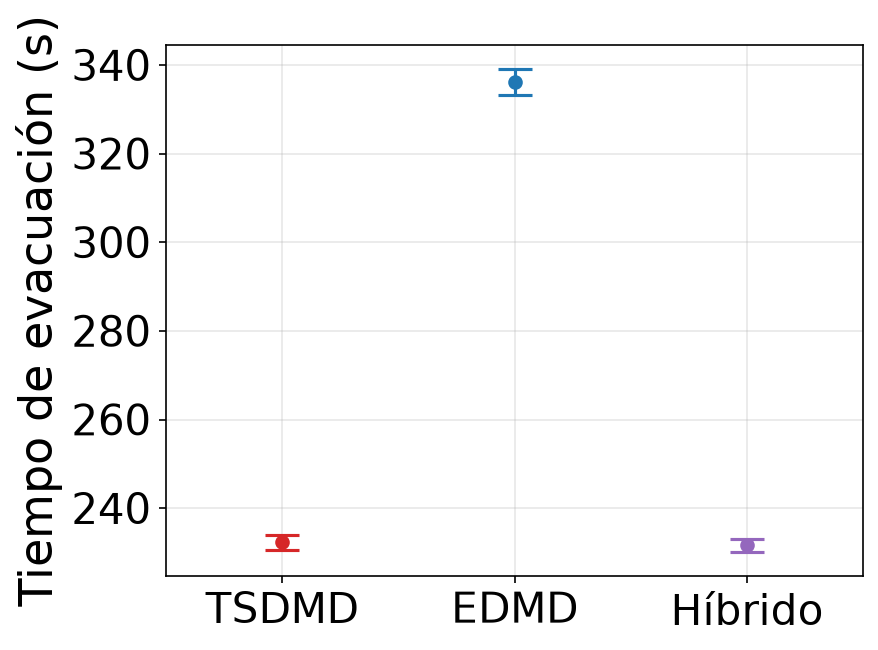
\includegraphics[width=\linewidth]{base_evacuacion.png}
		\end{column}
		\begin{column}{.48\textwidth}
			\centering
			\textbf{Tiempo de cómputo}\par\smallskip
			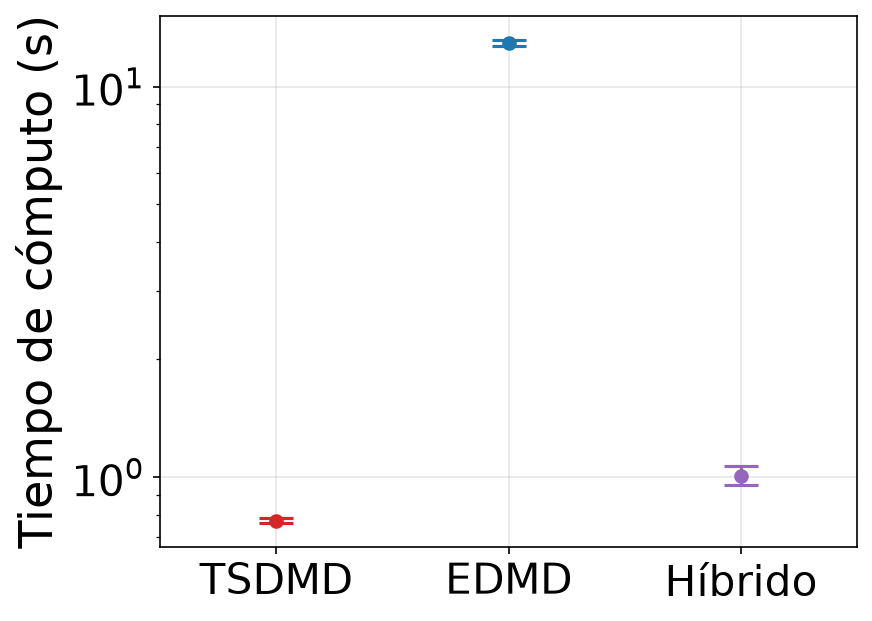
\includegraphics[width=\linewidth]{base_tiempo_computo.png}
		\end{column}
	\end{columns}
	
	\medskip
	\centering
	{\small\textcolor{magenta}{Cambiar las figuras de las barras}}
\end{frame}
\grafico{Anticipación: tiempo de evacuación}{barrido_evacuacion.png}{}
\grafico{Anticipación: tiempo de cómputo}{barrido_tiempo_computo.png}{}
\grafico{Distancia de cierre: participación de TS}{umbral_N500_fraccion_ts.png}{}
\begin{frame}{Distancia de cierre}
	\begin{columns}[T,onlytextwidth]
		\begin{column}{.48\textwidth}
			\centering
			\textbf{Tiempo de evacuación}\par\smallskip
			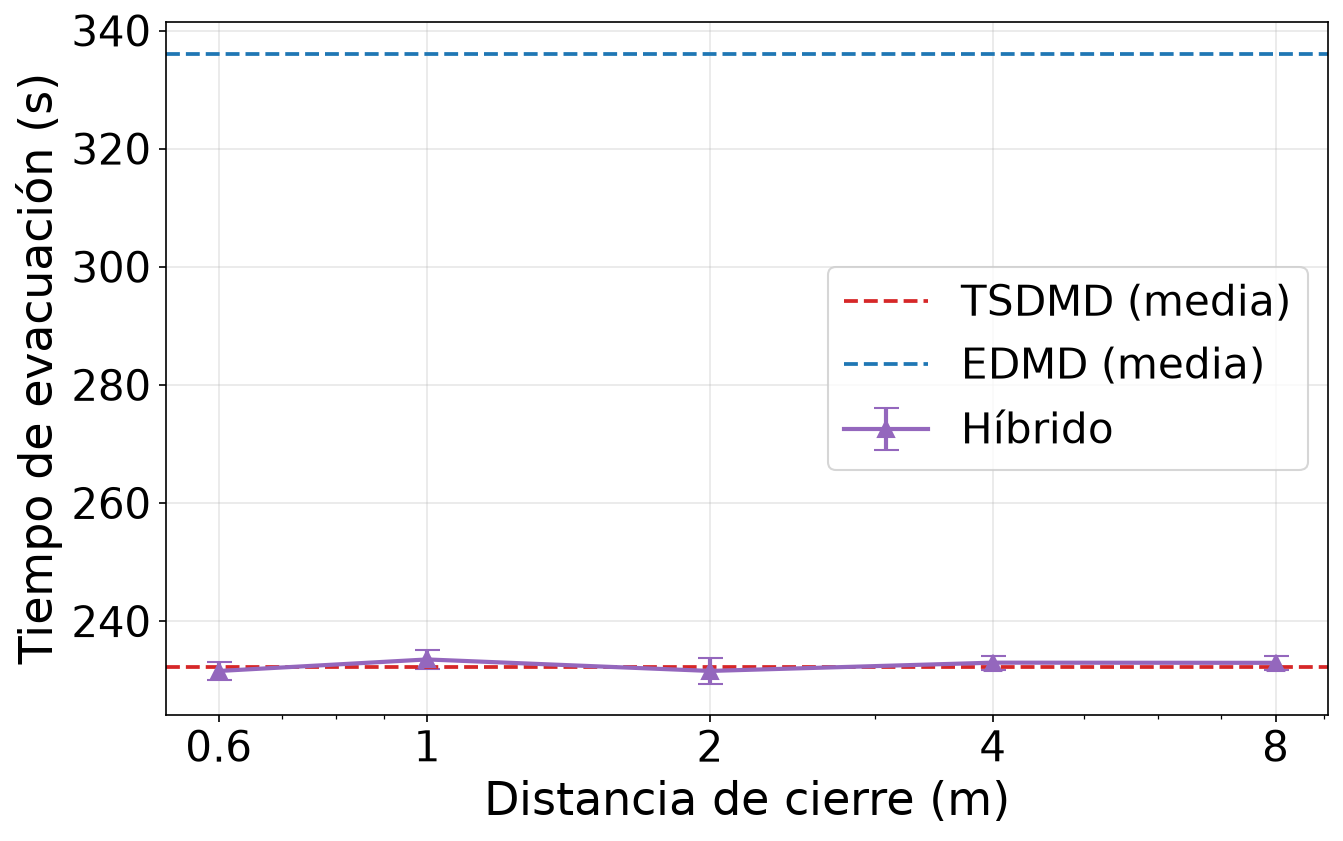
\includegraphics[width=\linewidth]{umbral_N500_evacuacion.png}
		\end{column}
		\begin{column}{.48\textwidth}
			\centering
			\textbf{Tiempo de cómputo}\par\smallskip
			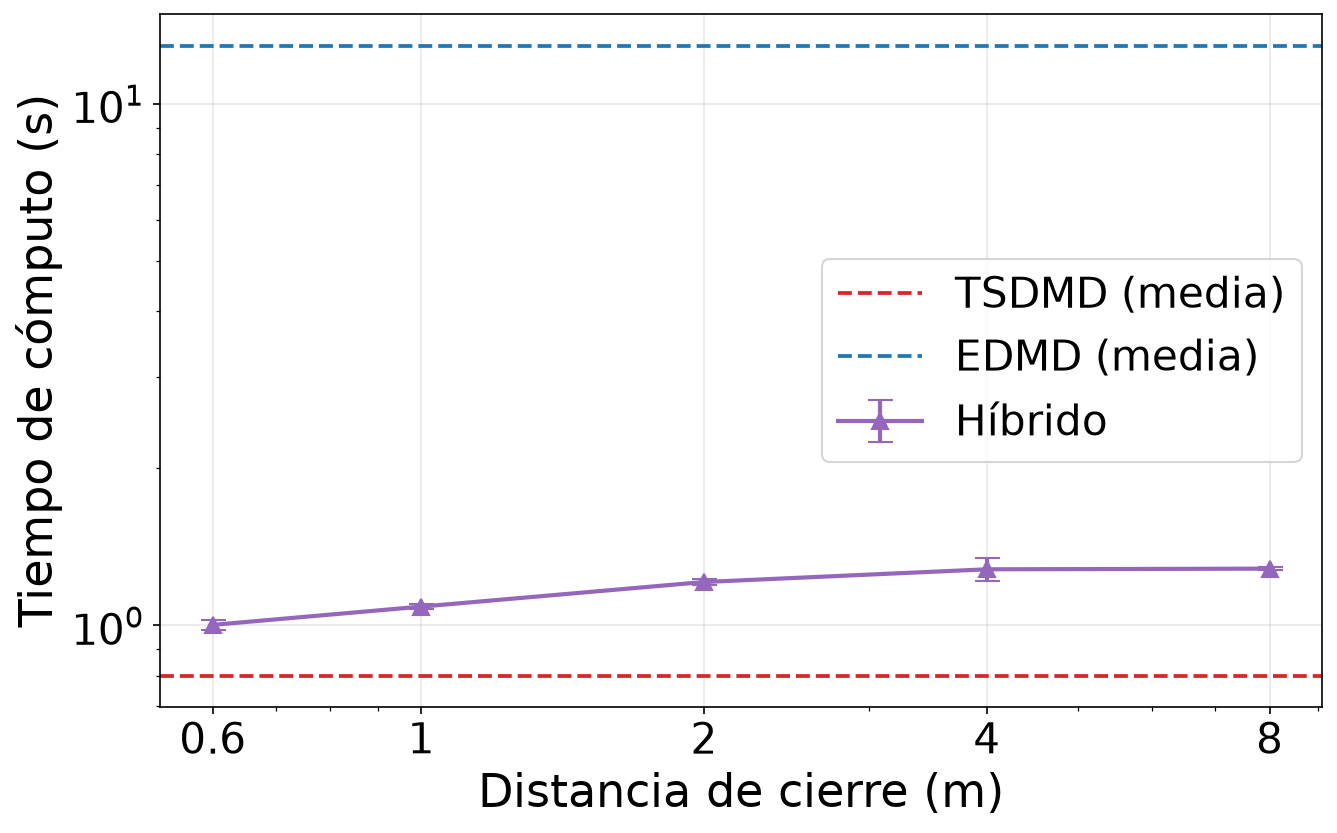
\includegraphics[width=\linewidth]{umbral_N500_tiempo_computo.png}
		\end{column}
	\end{columns}
\end{frame}
\grafico{Escalamiento a densidad inicial constante}{densidad_tiempo_computo.png}{}
\grafico{Escalamiento a tamaño de habitación constante}{lado_tiempo_computo.png}{}
\grafico{Costo relativo a TSDMD}{lado_costo_relativo.png}{}
% No hay en esta carpeta animaciones ni curvas temporales de los extremos de
% cada barrido. No presentar los tres videos base como si fueran esos estudios.

\section{Conclusiones}
\begin{frame}{Conclusiones}
\begin{itemize}\setlength{\itemsep}{9mm}
\item Caso base: TSDMD e híbrido dan $232\pm2\un{s}$; EDMD, $336\pm3\un{s}$.
\item El híbrido cuesta aproximadamente $1{,}3$ veces TSDMD; EDMD, $17$ veces.
\item Aumentar $d^*$ incorpora más agentes a TS y aumenta el costo en $N_0=500$.
\end{itemize}
% Cifras de base_resumen.csv; barras son desviación entre realizaciones.
% Cocientes descriptivos de medias, no ajuste ni test estadístico.
\label{finprincipal}
\end{frame}

\ifincluirapoyo
\apoyotrue
\section{Material de apoyo}
% Fuera del recorrido oral de 13 minutos. Todas las figuras restantes disponibles.
\grafico{Anticipación: fracción temporal TS}{barrido_fraccion_ts.png}{$N_0=500$, $L=50\un{m}$, $d^*=0{,}6\un{m}$.}
\grafico{Cierre con 10 agentes: evacuación}{umbral_N10_evacuacion.png}{$N_0=10$, $L=50\un{m}$, $k=1$.}
\grafico{Cierre con 10 agentes: cómputo}{umbral_N10_tiempo_computo.png}{$N_0=10$, $L=50\un{m}$, $k=1$.}
\grafico{Cierre con 10 agentes: fracción TS}{umbral_N10_fraccion_ts.png}{$N_0=10$, $L=50\un{m}$, $k=1$.}
\grafico{Cierre con 100 agentes: evacuación}{umbral_N100_evacuacion.png}{$N_0=100$, $L=50\un{m}$, $k=1$.}
\grafico{Cierre con 100 agentes: cómputo}{umbral_N100_tiempo_computo.png}{$N_0=100$, $L=50\un{m}$, $k=1$.}
\grafico{Cierre con 100 agentes: fracción TS}{umbral_N100_fraccion_ts.png}{$N_0=100$, $L=50\un{m}$, $k=1$.}
\grafico{Densidad fija: evacuación}{densidad_evacuacion.png}{$\rho_0=0{,}2\un{m^{-2}}$, $L=\sqrt{N_0/\rho_0}$.}
\grafico{Densidad fija: costo relativo}{densidad_costo_relativo.png}{$\rho_0=0{,}2\un{m^{-2}}$; cociente entre tiempos medios de motor.}
\grafico{Habitación fija: evacuación}{lado_evacuacion.png}{$L=50\un{m}$; densidad inicial variable.}
\grafico{TSDMD: realizaciones del caso base}{base_poblacion_tsdmd.png}{$N_0=500$, $L=50\un{m}$; diez realizaciones individuales.}
\grafico{EDMD: realizaciones del caso base}{base_poblacion_edmd.png}{$N_0=500$, $L=50\un{m}$; diez realizaciones individuales.}
\grafico{Híbrido: realizaciones del caso base}{base_poblacion_hybrid.png}{$N_0=500$, $L=50\un{m}$, $k=1$, $d^*=0{,}6\un{m}$; diez realizaciones individuales.}
\fi
\end{document}




